\section{Implementation}\label{sec:implementation} 
Detta kapitel innefattar en detaljerad beskrivning av implementeringen av systemet.
Implementeringen är uppdelad i olika delar som tillsammans utgör den övergripande lösningen. Varje del beskrivs i detalj, inklusive de tekniker, bibliotek och designval som gjorts under utvecklingen.
En översikt av systemet och dess komponenter presenteras i Figur \ref{fig:implementation_overview}.

\begin{figure}[H]
  \centering
  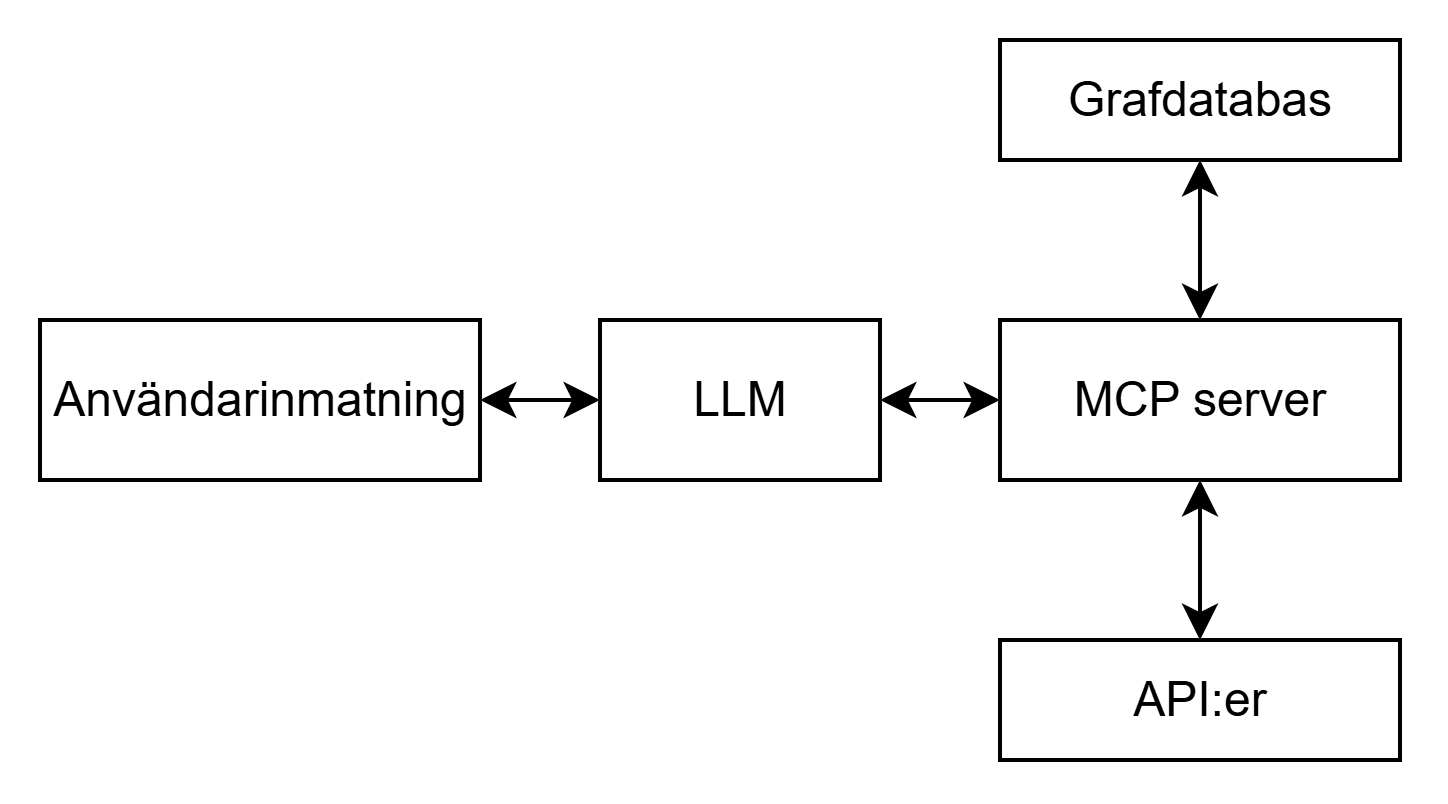
\includegraphics[width=15cm]{Figures/image.png}
  \caption{System översikt}\label{fig:implementation_overview}
\end{figure}

Figur \ref{fig:yyy} Visar en komplett bild över relationer mellan noder i grafdatabasen.

\begin{figure}[H]
  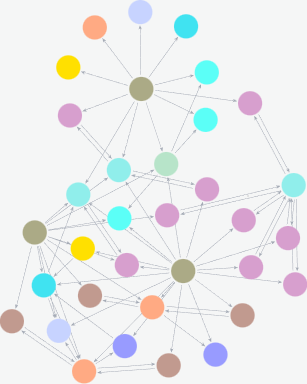
\includegraphics[width=\textwidth]{Figures/kg_quests/yyy.png}
  \caption{Fullständig bild över relationer mellan noder i grafdatabasen}\label{fig:yyy}
\end{figure}


% \subsection{System översikt}\label{subsec:overview1}


\subsection{Användarinmatning}\label{subsec:overview5}
Användaren interagerar med systemet genom att ställa frågor i ett naturligt språk. Användaren ställer frågor som "Vilka projekt har vi pågående?" eller "Vad står det i dokument x?", och behöver inte ha någon teknisk kunskap om hur systemet fungerar.

Dessa frågor ställs i ett användargränssnitt som tillhandahålls av Cherry Studio.

\subsection{LLM-kommunikation}\label{subsec:overview6}
Den AI-modell som används i systemet är GPT-5.4-mini, konfigurerad via Cherry Studio.
Modellen valdes för sin kombination av hög prestanda och låg kostnad, vilket möjliggjorde ett stort antal tester\cite{8}.

Modellen arbetar iterativt genom en så kallad agent-loop där den via MCP-servern kan anropa flera verktyg i sekvens.
Resultatet från ett anrop kan användas som indata till nästa, vilket är nödvändigt vid komplexa frågor som kräver information från flera delar av systemet.

\subsubsection{Systempromptar}
För att styra modellens beteende används en systemprompt som konfigureras i Cherry Studio.
De två lösningarna använder olika systempromptar eftersom de ställer olika krav på hur LLM:en ska resonera och använda verktyg.

\textbf{Grafdatabaslösningen:}
Systemprompten för grafdatabaslösningen fokuserar huvudsakligen på att vägleda LLM:en i hur Cypher-frågor ska formuleras.
Den instruerar modellen att alltid hämta databasens schema som första steg för att få tillgång till korrekta namn på entiteter och relationer innan en fråga formuleras.

Övrigt innehåller prompten instruktioner om namn matchning, tolkning av användarinmatning, felhantering och hur svaren ska formuleras.
Se Figur \ref{fig:p1} i Appendix \ref{sec:appA} för hela systemprompten som används.

\textbf{Den API-baserade lösningen:}
Systemprompten för den API-baserade lösningen fokuserar istället på att hjälpa LLM:en identifiera vilka verktyg som ska användas för en given fråga.
Eftersom det finns många verktyg kopplade till olika system och datakällor instrueras modellen om vilka verktyg som är lämpliga för olika typer av frågor, för att undvika onödiga eller felaktiga verktygsanrop.

Utöver detta innehåller prompten instruktioner om tolkning av inmatning, begränsningar i verktygsanvändning, felhantering och hur svaren ska formuleras.
Se Figur \ref{fig:p2} och \ref{fig:p3} i Appendix \ref{sec:appA} för hela systemprompten som används.

\subsection{MCP-servern}\label{subsec:overview2}
MCP-servern är en central komponent i systemet som fungerar som en mellanhand mellan LLM'en och de externa verktygen. 
Istället för att LLM'en kommunicerar direkt med databasen eller API:erna sker istället all kommunikation via MCP-servern, som i sin tur kommunicerar med de externa verktygen.

Servern exponerar funktionalitet i form av verktyg (tools), som LLM'en anropar. Varje verktyg representerar en specifik operation, exempelvis hämta schema från grafdatabasen eller hämta senaste uppdateringen från ett specifikt dokument.
Detta innebär att språkmodellen inte behöver känna till detaljer kring hur data lagras eller hämtas, utan endast vilka verktyg som finns och hur de används.

Implementationen av MCP-servern är baserad på ett HTTP-gränssnitt där inkommande förfrågningar hanteras via en endpoint.
Servern upprättar en session per startad chatt, vilket möjliggör en kontinuerlig kommunikation tills att servern stängs av.
Verktygen registreras vid uppstart av servern och görs då tillgängliga för språkmodellen. Vid testning och jämförelse av de olika arkitekturerna registreras endast de verktyg som tillhör respektive lösning, de andra kommenteras tillfälligt bort.

Detta möjliggör en enhetlig kommunikationskanal där LLM'en använder samma gränssnitt oavsett om data hämtas från en databas eller API:er.
Det gör det också möjligt att enkelt byta ut och lägga till verktyg utan att behöva ändra något annat i systemet.

\subsubsection{Grafbaserade lösningens verktyg}
Strukturen för dessa verktyg är relativt simpel.
 Det finns ett verktyg som returnerar hela schemat i grafdatabasen och ett verktyg som tar emot en cypher-fråga och returnerar resultatet av denna fråga.

Det första verktyget har som syfte att ge LLM'en en överblick över hur data är strukturerad i grafdatabasen.
Det får tillgång till information om vilka entiteter och relationer som finns, samt vilka attribut som är kopplade till dessa.
Syftet är att LLM'en ska kunna använda denna information för att få de korrekta namnen på entiteter och relationer, och för att då kunna formulera cypher-frågor som kan returnera det som efterfrågas.

Det andra verktyget används för att exekvera de genererade cypher-frågorna mot grafdatabasen. 
LLM'en formulerar en cypher-fråga baserat på användarens fråga och den information den har om databasens struktur.
Resultatet från frågorna returneras sedan till LLM'en i ett strukturerat JSON-format som den sedan använder för att formulera sitt svar till användaren.

Genom denna design ges LLM'en en hög grad av flexibilitet och kontroll, då den själv bestämmer vilka vägar den ska traversera i grafen för att hitta och hämta den information som efterfrågas.
Samtidigt innebär det att LLM'ens förmåga att förstå relationerna i grafen för att kunna generera en giltig och korrekt cypher-fråga är avgörande för att lösningen ska fungera.

\subsubsection{API-baserade lösningens verktyg}
I den API-baserade lösningen är verktygen mer specifika och inriktade på att hämta information från specifika API:er.
Totalt finns 20 verktyg fördelade över de tre systemen: 8 för GitHub, 7 för Confluence och 5 för Slack.

GitHub-verktygen täcker bland annat hämtning av repositories, issues, commits och aktiva användare.
Confluence-verktygen hanterar hämtning av spaces, dokument, författare och sökning på nyckelord.
Slack-verktygen täcker hämtning av användare och meddelanden från specifika kanaler med mera.

Dessa verktyg kapslar in API-anrop och returnerar resultatet i ett strukturerat format som LLM:en sedan kan använda för att antingen anropa ett annat verktyg eller formulera ett svar till användaren.

Jämfört med grafdatabaslösningens 2 verktyg kräver denna lösning alltså 20 verktyg för att täcka samma informationsbehov.
Detta innebär att LLM:en måste identifiera rätt verktyg för varje fråga, och att frågor som berör flera system kräver en sekvens av anrop där modellen själv kombinerar informationen.

\subsection{Grafdatabasen}\label{subsec:overview3}
Den grafbaserade lösningen bygger på en grafdatabas som implementerats i Neo4j.
Grafdatabasen används för att representera organisationens struktur och aktiviteter på ett sammanhängande sätt för att möjliggöra att information kan hämtas genom traversering av relationer mellan entiteter.

\subsubsection{Datamodell}

Grafen består av flera typer av noder som representerar delarna i organisationen. Dessa inkluderar \textit{Person}, \textit{Team}, 
\textit{Project}, \textit{Repository}, \textit{Issue}, \textit{Commit}, 
\textit{SlackChannel}, \textit{Post}, \textit{ConfluenceSpace}
\textit{Document}. Varje nod innehåller egenskaper såsom id, namn, tidsstämplar med mera.

Relationer används för att koppla samman dessa noder. Namnet på dessa relationer spelar stor roll eftersom det är de som LLM:en utgår från när cypher-frågan genereras.
Exempelvis kopplas en person till ett team via relationen \textit{MEMBER\_OF}, och till ett dokument via relationen \textit{AUTHORED}, medan ett inlägg i en slackkanal kopplas mellan inlägget och kanalen via relationen \textit{HAS\_POST}.
Dessa skapar en sammanhängande struktur där information kan följas mellan olika delar av systemet.

\subsubsection{Implementation i Neo4j}
Grafen skapades genom cypher-frågor där noder och relationer definierades explicit.
Data lagras i Neo4j och nås via databasanslutningen som används av MCP-servern.

\subsection{API-baserade lösningen}\label{subsec:overview4}

Den API-baserade lösningen implementerades genom att integrera systemen GitHub, Slack och Confluence via deras API:er.
Till skillnad från grafdatabaslösningen lagras ingen data centralt, utan all information hämtas dynamiskt via respektive systems API.

\subsubsection{Datakällor och struktur}
De externa systemen representerar olika delar av organisationens struktur och aktiviteter.
GitHub används för att hämta information om repositories, issues, commits och aktiva användare, Slack används för att hämta information om kanaler och inlägg i dessa, och Confluence används för att hämta dokumentation.

Varje system har sin egen datastruktur och sina identifierare. Detta innebär att det inte finns någon gemensam modell som binder samman en person från github till ett meddelande i Slack.
Detta innebär att samma entitet förekommer i flera system utan direkt koppling.

\subsubsection{Implementation av API-integrationer}

API-integrationerna implementerades genom separata funktioner som kapslar in anrop till respektive system.
Dessa funktioner används av MCP-servern och exponeras som verktyg till LLM'en. Varje verktyg är anpassad efter en specifik typ av data, exempelvis hämta information från ett specifikt repository.

Resultaten från dessa anrop returneras i ett strukturerat format, vilket gör det möjligt för LLM'en att jobba vidare med informationen.

\subsubsection{Integration med MCP och LLM}

LLM'en interagerar med de externa systemen via MCP-servern genom att 
anropa flera olika verktyg beroende på användarens fråga. Till skillnad från 
grafdatabaslösningen, där en enskild fråga kan räcka, kräver denna lösning ofta 
en sekvens av verktygsanrop.

Modellen använder resultatet från ett verktyg som indata till nästa steg i 
processen, vilket möjliggör att information från flera system kan kombineras. 
Denna iterativa process hanteras inom agent-loopen och fortsätter tills modellen 
har tillräckligt med information för att generera ett svar.

\subsection{Evalueringsupplägg}\label{subsec:eval_setup} 

För att utvärdera de två lösningarna har 15 testfrågor definierats, där frågorna varierar i komplexitet.
Varje fråga körs i en ny session för att inte tidigare frågor och svar ska påverka LLM'ens resonemang.

Vid varje tests mäts korrekthet, tid, antal verktygsanrop samt om modellen behöver ställa följdfrågor.

Mätningen om svarstid sker från att användarens fråga är skickad tills dess att ett färdigt svar är genererat.

Testmiljön består av den implementerade MCP-servern tillsammans med respektive lösning, där endast relevanta verktyg för den lösningen är aktiverade.


